\chapter{Towards measuring Tan's contact in 1D gases}

\section{Tan's contact for 1D gases}

To understand what Tan's contact is, we consider two atoms with contact interactions in 1D. 

\section{Theoretical study}

\subsection{Effect of temperature}

\subsection{Effect of the interaction parameter}

\section{Experimental realisation of 1D gases with the optical lattice}

The main idea to experimentally study 1D physics is to ``freeze'' the degrees of freedom of the atoms in two directions of space. To do so, the easiest solution is to use a harmonic trapping potential with trapping frequencies $\omega_{\perp}$ high enough so that the energy difference $\Delta E =\hbar \omega_{\perp}$ between the ground-state and the first excited state is much larger than the typical energy of the atoms $\Delta E \gg \kB T, \mu$. Such high trapping frequencies are accessible in our experiment thanks to the optical lattice. Instead of using the 3 pairs of countra-propagating beam as we did so far, we use only 2 to produce a 2D lattice. Interestingly, the total laser power is divided amongst 2 pair of beams instead of 3, meaning that we can reach much higher values of the lattice depth, typically up to $s=30$. In the direction where there is no lattice, the trapping potential results from the Gaussian shape of the beams and has a trapping frequency $\omega_{\rm{1D}} =2 \pi \times 140 \sqrt{s} = 2 \pi  \times 713 \ \rm{Hz}$ for $s=26$. In the other 2 directions, the trapping frequency is however very large as a result of the lattice interference pattern $\omega_{\perp} \simeq 200 \ \rm{kHz}$, which is much larger than the energy of the atoms $\kB T, \mu \simeq 25 \ \rm{kHz}$ with typical experimental parameters.

\begin{figure}
    \centering
    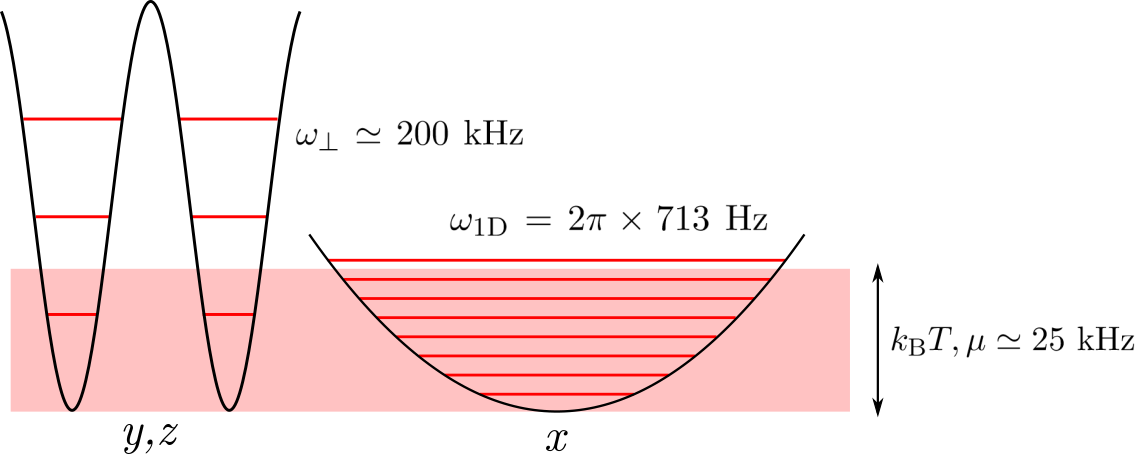
\includegraphics[width=0.9\textwidth]{Fig/Chapter5/1D_config.png}
    \caption{Configuration of the optical lattice to produce 1D tubes. In the transverse direction, the lattice interference pattern creates a confining potential that can be approximated to a harmonic potential near the center of the site. The trapping frequency is high enough so that the degree of freedom of the atoms in these directions is ``frozen''. On the other hand, the lattice is absent in the longitudinal direction and the trapping frequency only results from the Gaussian shape of the beams. This is the 1D direction.}
    \label{fig:my_label}
\end{figure}


Using the optical lattice in this configuration then allows us to emulated 1D physics. The main drawback of this method is that we end up with an array of 1D gases rather than a single one, complicating the comparison with theory.

\subsection{Independence of the tubes}

In order to properly observe 1D physics, it is crucial that all the 1D tubes are independent from one another, \ie no coherence subsists in the transverse directions. This is true when the typical timescale \NOTE{faire cette section}

\subsection{Number of atoms in the 1D tubes}

The major difficulty comes from the fact the atom number varies from one 1D tube to another. To determine the atom number distribution, we first need to determine the density profile of the cloud in the 2D lattice.

To do so, we first remind that under the Thomas-Fermi approximation (\NOTE{ref}), the density profile of a BEC in a 3D harmonic potential writes:

\begin{equation}
     n(\bm{r}) = \frac{\mu}{g} \, \left[ 1 - \left( \frac{x}{R_x} \right)^2 - \left( \frac{y}{R_y} \right)^2 - \left( \frac{z}{R_z} \right)^2 \right]
\end{equation}

\noindent where $R_i = \sqrt{\frac{2 \mu}{m \omega_i^2}}$ is the Thomas-Fermi radius in direction $i$. Under the mean-field approximation, the chemical potential is:

\begin{equation}
     \mu = \frac{\hbar \bar{\omega}}{2} \left(  15 N_{\rm{tot}} \frac{a_s}{a_{\rm{ho}}}\right)^{2/5}
\end{equation}

with $\bar{\omega}=\omega_x \omega_y \omega_z/3$ the average trapping frequency, $a_s$ the scattering length and $a_{\rm{ho}}=\sqrt{\hbar/m \bar{\omega}}$ as previously seen on different occasions in this manuscript.

Similarly to the method developed in \ref{sec:rescaled_interaction}, we rescale $\mu$ to account for the presence of the 2D lattice with:

\begin{equation}
    \tilde{\mu} = \frac{\hbar \bar{\omega}}{2} \left(  15 N_{\rm{tot}} \frac{\tilde{a}_s}{a_{\rm{ho}}}\right)^{2/5}
\end{equation}

\noindent where $\tilde{a}_s= a_s \left(d \int_0^d |u_{0,0} (x)|^4 \mathrm{d}x \right)^2$ is the rescaled interaction strength, with the notable difference that we are using here a power 2 instead of power 3 in \ref{sec:rescaled_interaction} as we use here a 3D lattice. \NOTE{vérifier}

\NOTE{expliquer algo nombre d'atomes par tubes}

\section{Detection of large momentum components}

While the great sensitivity of the $\He$ detector is perfectly suited to detect the very low density $\kmf$ momentum tails, the size of the MCPs limits the range of detector. From the work \cite{xu2015universal}, we obtain that the $\kmf$ decay should start around $k_0 \sim 1.6 \times \rho_{\rm{1D}}(0)$ \NOTE{blah blah chiffres}.

\subsection{Magnetic gradient and displacement procedure}

One solution to this issue is to give the entire cloud a momentum kick in the first instants of the TOF to artificially change the momentum range of the $\He$ detector. With our experimental setup, the easiest way to do so is to create a magnetic gradient to apply a magnetic force on the atoms during a time $t_{\rm{grad}}$ before transferring them to the $m_j=0$ sub-state. 

This technique however brings some experimental complications as the population transfer cannot be done immediately after turning off the trap. As a matter of fact, the atoms starts moving during the time $t_{\rm{grad}}$ and will therefore be at different positions when the transfer is performed. The problem comes from the fact that there is a slight inhomogeneity in the bias field along direction $x$ used to set the energy difference between the sub-states $m_j=0$ and $m_j=1$. This means that the resonance condition for a Raman or RF transfer depends on the initial momentum of the atoms, with the consequence that we cannot properly transfer the whole cloud to $m_j=0$ with a simple single frequency Rabi pulse.

To solve this issue, \NOTE{expliquer rapidement sweep}. We understand however that it is increasingly difficult to fulfill the adiabatic condition for all momentum classes if the spread in resonance frequencies is too high. We therefore need to devise a displacement sequence as short as possible to minimize the distance travelled by the atoms before the transfer, as well as to make sure that the magnetic gradient is properly turned off not to further increase the field inhomogeneity.

The procedure is represented on Fig.-\ref{fig:displacement_sequence}. Right after the lattice is turned off, we increase the current in the MOT coils to produce the magnetic gradient. The MOT coils are indeed the coils with which we can produce the stronger gradient, reducing the time during which we need to apply it to reach the proper momentum shift. However, the current in the MOT coils typically needs around $10 \ \rm{ms}$ to reach the highest possible values, which is already too long. We then set the command voltage $V_{\rm{command}}$ to be close to the highest possible value, let the current increase for $t_1 = 1 \ \rm{ms}$ and then set the command to $0$ and let the current decay for $t_2-t_1=13 \ \rm{ms}$ \NOTE{check numbers} until it is fully turned off. After that, we finally perform the population transfer and let the atoms fall unto the MCP. The momentum displacement of the cloud can be set by changing the command voltage $V_{\rm{command}}$.

\begin{figure}
    \centering
    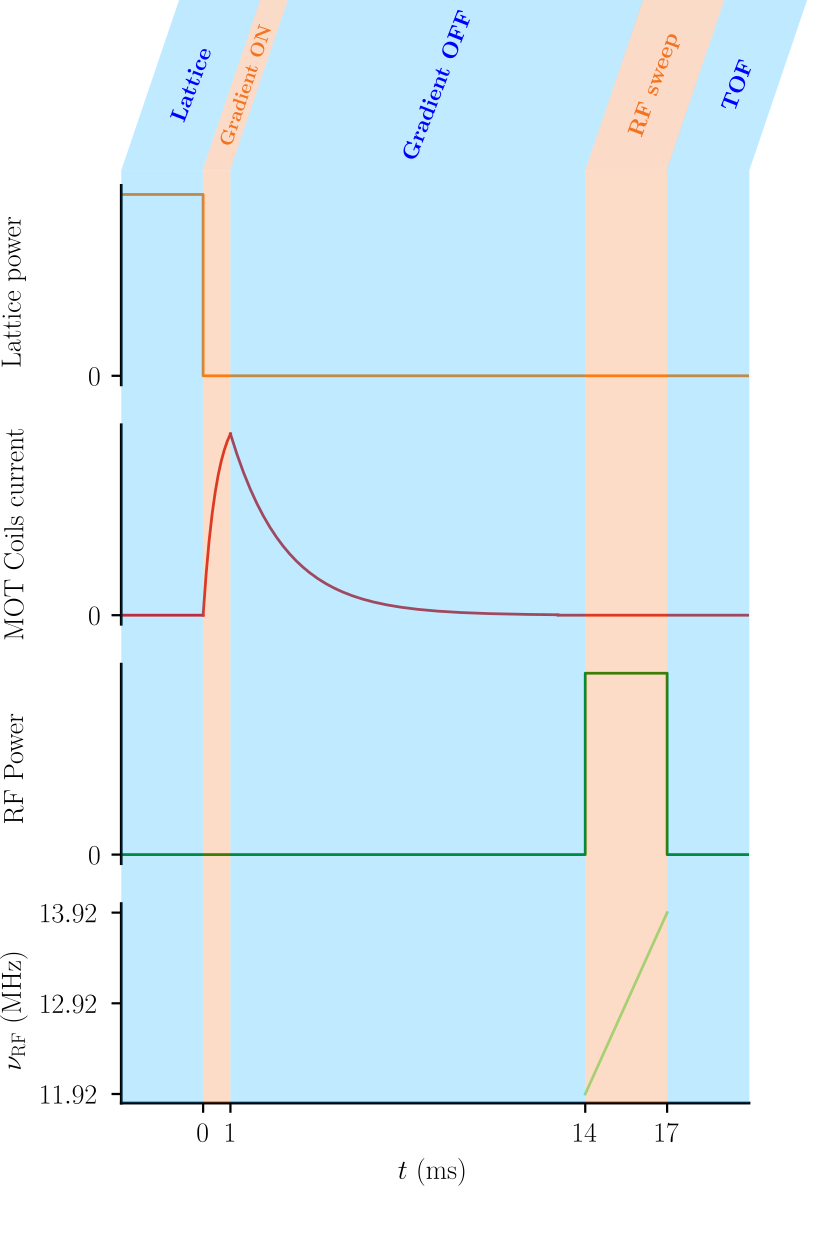
\includegraphics[width=0.8\textwidth]{Fig/Chapter5/displacement_sequence.png}
    \caption{Experimental sequence to shift the entire momentum distribution so that the $\kmf$ tails fall unto the $\He$ detector.}
    \label{fig:displacement_sequence}
\end{figure}

\subsection{Benchmarking with 3D lattice gases momentum distribution}

To test that our method does not induce any distortion of the momentum distribution, we benchmark it with 3D lattice gas momentum distribution slightly above the Mott critical point so that the momentum distribution has a wide background but still sharp diffraction peaks. This allows to check for distortion at high momentum values, while making more precise measurements with the narrow diffraction peaks \NOTE{vraiment pas ouf}.





\section{Experimental study}

\subsection{Measurement of the temperature}

\subsection{First extracted values of the Tan's contact}

\subsection{Comparison with QMC calculations}

\section{Discussion of the preliminary results}